The Deep Underground Neutrino Experiment (DUNE) \cite{if:DUNE} will utilize massive LArTPC's to measure the CP violating phase ($\delta_{CP}$) in the neutrino sector and determine the neutrino mass hierarchy. DUNE will use a high power proton beam capable of producing a large number of neutrinos and antineutrinos directed from Fermilab towards massive underground LArTPC detectors located in the Sanford Underground Research Facility (SURF) in Lead, South Dakota. By measuring the asymmetry between appearance of $\nu_{e}$ from a beam of $\nu_{\mu}$ compared to the appearance of $\overline{\nu}_{e}$ from a beam of $\overline{\nu}_{\mu}$ as well as the precise measurement of the $\nu_{e}$ energy spectrum at the far detector, the measurement $\delta_{CP}$ and the determination of the neutrino mass hierarchy can be done in the same experiment. In order to achieve these goals, DUNE will require three essential components:
\begin{itemize}
\item[1)] \underline{High power neutrino beam:}

A neutrino beamline designed to provide sufficient intensity in an energy range to enhance the sensitivity to the first and second oscillation maxima. The beam comes from a conventional, horn-focused neutrino beamline generated from 60 GeV - 120 GeV protons from the Fermilab Main Injector designed for initial operation at proton-beam power of 1.2 MW with the capability to support an upgrade to 2.4 MW. The beam will be sign-selected to provide separate neutrino and antineutrino beams to enable measurement of $\delta_{CP}$ and the neutrino mass hierarchy as well as precision measurements of oscillation parameters.

\item[2)] \underline{Large mass underground far detector:}

The far detector is designed to be a 40 kt LArTPC consisting of four 10 kt detectors. These detectors will be stationed 4850 feet below the surface in caverns located at SURF in order to reduce the number of cosmic rays in time with the neutrino beam to $\sim$1$\%$ of the expected background. These detectors are capable of precision ${\nu}_{\mu} / \bar{\nu}_{\mu}$ and ${\nu}_{e} / \bar{\nu}_{e}$ identification and energy measurements to provide definitive measurement of $\delta_{CP}$ and mass hierarchy.

\item[3)] \underline{Precision near detector:}

The near detector, which is exposed to an intense flux of neutrinos, also enables a wealth of fundamental neutrino interaction measurements. The current reference design for the DUNE near detector includes a NOMAD-inspired \cite{if:nomad} fine-grained tracker consisting of a 3.5 m$\times$3.5 m$\times$6.4 m central straw-tube tracker, a lead-scintillator sampling electromagnetic calorimeter, a 4.5 m$\times$4.5 m$\times$8.0 m large-bore warm dipole magnet surrounding the straw tube tracker and the calorimeter providing a magnetic field of 0.4 T, and RPC-based muon detectors sandwiched in the steel of the magnet as well as upstream and downstream of the tracker.

\end{itemize}

In the subsequent sections, we describe in detail the project listed in the strategic plans.   The primary goal of the projects listed in this section are to ensure the group to play leadership role in construction of first two 10 kt modules of DUNE as well as in physics topics of the group's interest. 

%
% ==========  ProtoDUNE Single Phase
%
\subsection{ProtoDUNE Single Phase APA QA/QC (PI: Asaadi)}~\label{sec:proto-dune-sp-apa}

Given that the highest priority of DUNE is to establish and demonstrate the functionality of its baseline technology, namely the single phase LArTPC, Asaadi will be focusing on the quality assurance, quality control, and commissioning of the anode plane assemblies (APA's) for protoDUNE SP. This work will help building up infrastructure, expertise, and capabilities necessary to contribute and lead in the DUNE SP far detector construction.  He plans on resident at CERN in the first half of 2018 coordinating with Yu in order to make contributions to both protoDUNE experiments and to manage UTA I.F. personnel during the construction and installation period of protoDUNE experiments. 

The QA/QC testing plan being developed in collaboration with Univeristy of Wisconsin's Physical Science Laboratory (PSL, who are building the APA's) and the DUNE APA conveners (Tim Bolton and Mitch Soderberg) will be first executed at the construction site (PSL) and then again at CERN prior to installation. UTA members will be present during the testing both at PSL and CERN to aid in the successful installation and commissioning of the SP protoDUNE experiment. The testing plan developed for the SP is intended to have applicability to UTA's efforts on the DP, where common technology is present. 

%
% ==========  ProtoDUNE Dual Phase
%
\subsubsection{Field Cage for protoDUNE Dual Phase}
Field cages provide uniform electric fields for ionization electrons to drift to anodes for the detection in the Time Projection Chamber.
The baseline design for DUNE LAr TPC is that of the single phase in which the ionization electrons created by the secondary particles 
resulting in neutrino-nucleon interactions drift in LAr and get detected on the anode plane that resides inside the liquid phase of argon.  An alternative technology is the LAr TPC that the ionization electrons drift through LAr but then extracted through the strong extraction field at the top of the liquid and detected in the anode in gaseous phase of argon after a signal amplification via an large area gas electron multiplier (LEM), hence the dual phase.

During the period of his sabbatical stay at CERN, Yu has begun to work on WA105, a dual phase $6m\times 6m\times 6m$ prototype testing project at CERN through the participation in the smaller prototype cosmic ray detector in $1m\times 1m\times 3m$.  This work provided an opportunity for UTA IF group to join WA105 as the first U.S. group and to position itself well to play a leading role in dual phase.   While dual phase technology is currently at a lower priority to the single phase LAr TPC, it is clear that U.S. groups' participation in alternate technology is beneficial in many perspectives, including that of strengthening the international nature of DUNE collaboration an essential ingredient in its success.

As the schedule for DUNE experiment and for the two protoDUNE experiments get clearer, it became apparent that UTA will be able to play an importnat role in design and construction of these experiments.   The overarching strategy in identifying the construction was to ensure UTA's contribution to any of the two protoDUNE experiment would aim to direct participation in DUNE from the first 10kt module in early 2020s.  One such component easily identifiable is the field cage for which the collaboration is targetting to utilize as much common components as possible for single phase and dual phase protoDUNE detectors.    With this premise, Yu has discussed with the DUNE management and has agreed to take the responsibility in design and construciton of dual phase field cage together with the University of Zurich group.    

Figure~\ref{fig:if-dp-fc} shows the current conceptual design of the field cage for the dual phase protoDUNE experiment.   The primay concept of this field cage is to use compartmentalized structure of submodules that consist of several straight profiles to provide voltage differentials for the generation of uniform fields.   The use of straight profiles made of either aluminium or stanless steel makes the preassembly and shipment of submodules convenient.   Each of these submodules will be prepared to the quality to hold high voltages at 180kV (for single phase) or  360kV (for dual phase) over the drift length.  
\begin{figure}[htb]
\centering
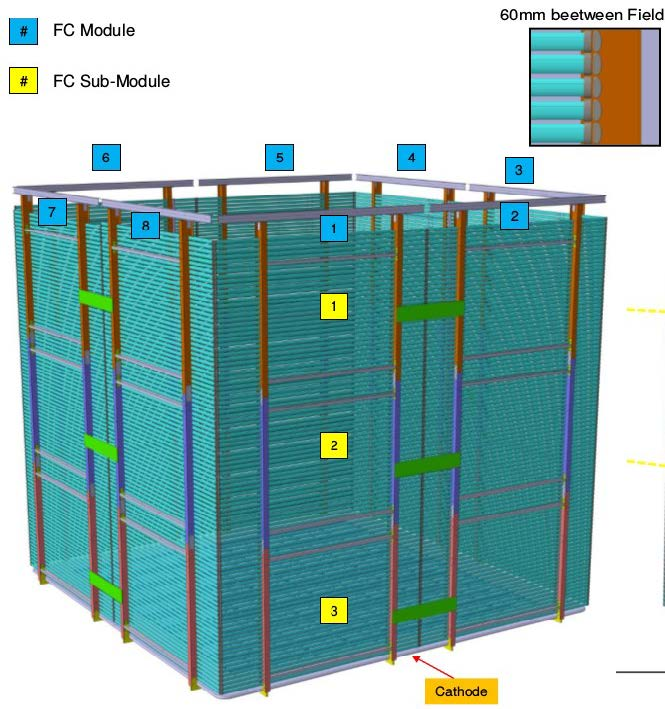
\includegraphics[width=0.80\textwidth]{images/if-dp-fc.jpg}
\caption[]{Conceptual skematic drwaing of the field cage assembly for dual phase protoDUNE.}
\label{fig:if-dp-fc}
\end{figure}

At present, it has been agreed that either CERN or Fermilab will be responsible for purchasing and production of the necessary mechanical parts, including the I--beams that act as the spine of the submodule and the each profile.  The project funds will pay for the purchase electrical parts - voltage divider resisters and varisters for surge arresting - and the production of electronic boards the field cage.  UTA will work with the single phase field cage group, including BNL team, and the single phase field cage electronics group at Louisiana State University as well as the University of Zurich group on design of both the mechnical and electrical part of the dual phase field cage.   We will be responsible for preassembly of the field cage submodules, mouting of the electric boards, testing of each submodules and performaning functional prototype testing with as large a field cage as possible before shipping the dissembled submodules out to CERN for installation.

For the completion of the design of the dual phase field cage, our postdoctoral fellow, Animesh Chatterjee will be stationed at CERN starting from October 2016 through mid January 2017.   During this period, Chatterjee will work with the ETH and CERN groups to finalize both mechnical and electrical design of the field cage for dual phase protoDUNE and ensure as much a commonality as posisble with that of the single phase.  Once these design parameters are agreed with the single phase field cage groups, a production could proceed.  The parts for the dual phase field cage will be shipped to UTA for the clean up and preparation of each of the parts, assembly of submodules, mounting of electrical components, and electrical and mechanical testing for a submodule qualification. A sizeable functional prototype field cage of size $6m\times 6m$, an electrically independent unit, will be put together and be subject under high voltage, though it may not be as high as 360kV given that the testing will be performed in air.  Once the functional testing completes, the functional prototype will be disassembled and shipped to CERN for the installation.

Since protoDUNE time scale has a hard limit of completing the beam data taking before CERN shutdown in 2018, it is essential for our group to operate under this time restriction in mind as presented in the strategic plan in section~\ref{ss:trategic-plan}.  To meet these goals, Yu plans on staying out at CERN in fall 2017, thanks to the remaining funds from the agreements with LAPP and ETH which covers costs for local stay at CERN and the teaching buyout.   A UTA postdoctoral fellow will also be stationed out at CERN together with a graduate student to help with both single and dual phase protoDUNE installation and commissioning.   Yu will then return to the U.S. at the end of year 2017 and Asaadi will be stationed out at CERN for the first half of 2018 to continue fulfilling our responsibilities in both the protoDUNE experiments.

At the time of writing this renewal proposal, the dual phase protoDUNE field cage group is working closely with the group for the single phase to agree on common design parameter for mechnical and electrical components of the field cages, such as the dimension of each profile bars of the field cage, the material, the electrical board design, quality and tolerance of resisters and varisters, etc. 

%
% ==========  DUNE BSM group
%
\threehead{Beyond the Standard Model physics group leadership (PI: Yu)}~\label{sec:dune-bsm}
In addition to the standard neutrino physics topics, neutrino mass hierarchy and CP violation phase measurements in the neutrino sector, the required high intensity proton beams provide ample opportunities for DUNE to look for physical phenomena beyond the Standard Model. UTA has been the leading proponent in searching for Low mass Dark Matter (LDM) in high intensity proton beams from the start of the IF group in 2014. For this work, Yu has been leading the BSM physics working group of DUNE since its inception in 2015 and has grown the group to play a significant role within the collaboration. Yu plans on ensuring various BSM topics be included in the DUNE Technical Design Report (TDR) to be released in summer 2019.

In order to coordinate the group in an effective manner, Yu quickly organized the group into five subgroups based on primary physics interests and to provide necessary simulation and analysis tools specialized to support the BSM group physics analyses.
The five subgroups are the simulation and software group led by UTA's postdoctoral fellow, Chatterjee and four physics subgroups that cover LDM search (Yu, Chatterjee), the Sterile Neutrino Search, the Non-standard Neutrino Interactions searches and Heavy Neutrino searches. Additional physics topics would continued to be added to the group's interest but these four physics topics are the primary topics to be studied in the coming 1.5 to 2 year time scale with the goal to provide the results for DUNE TDR.
In preparation for TDR, the group plans on producing a document that contains the initial list of topics and tasks to complete to provide
sensitivity studies for TDR, along with the milestones for the group to follow, by the end of 2016. 

\threehead{Search for Low-mass Dark matter (PI: Yu)}
As described in Section~\ref{sec:strategic-plan}, high power proton beams necessary for high flux neutrino beams enable experiments to search for BSM phenomena.  The particular interest of our group is the potential for discovering LDM particles in high precision detectors. The LDM particles produced in the target through the decay of a mediator (e.g. dark photons) can be detected through neutral-current like interactions either with electrons or nucleons in the detector. Since the signature of DM events looks just like those of the neutrinos, the neutrino beam provides the major source of background for the LDM signal. 

Several ways have been proposed to suppress neutrino backgrounds by using the unique characteristics of the DM in the beam. Since DM will travel much slower than the neutrinos, due to its much higher mass, the arrival time of the LDM signal in the detector can be used to distinguish LDM from neutrinos.  Additionally, since the electrons struck by LDM will have a more forward direction than those from neutrino interactions and the scattering angle of the electrons from the interaction may be used to reduce backgrounds, taking advantage of fine angular resolution a LArTPC can provide. Finally, a special run can be devised to turn off the focusing horn to significantly reduce the charged particle flux that will produce neutrinos. A major goal of the study currently underway is ensure the inclusion of the sensitivity estimate in a near detector to DUNE TDR.

Finally, given the large mass of ICARUS detector and its off-axis location with respect to the NuMI target, it may also be feasible to search for LDM from the NuMI beam.  Since ICARUS is single phase LArTPC, such a study in ICARUS will enable a more realistic and systematic study in preparation for the search in DUNE. 

%Given these new theoretical background, high intensity proton beams that are needed for DUNE will provide sensitivity to mass ranges inaccessible at direct-detection experiments such as CDMS and XENON~\cite{Aprile:2012nq}.  
%We believe this effort has the potential of expanding DUNE's physics motivation beyond neutrinos, super-novae, and proton decays. For this work, Yu and the postdoctoral fellow, Chatterjee have been working on integrating the existing MadGraph~c\cite{if:madDraph} based simulation package into the existing LBNE/DUNE fast simulations. A version of this package has already been prepared for Non-Standard Model Neutrino Interaction studies for the DUNE BSM physics group.  Our Ph.D. student has been working on data analysis of MiniBooNE beam dump experiment for feasibility study.
%We are working to write a Monte carlo code for the search of sub-GeV dark matter using LBNF beam line at DUNE experiment. Models of sub-GeV dark matter typically involve a scalar or fermionic dark matter and vector or scalar mediator. In our model we have considered 120 GeV proton scattering with a target produces dark matter. We have also calculated the neutrino background signal at position of the DUNE near detector location. We have tried to estimate the optimum angle between the detector location and beamline for which we get minimum neutrino background. Our main goal is to design a software framework for DUNE beyond standard model group. We are now in a stage of getting final simulation results about NSI parameter. We are also in a processes of getting preliminary result of dark matter search study.
%
% ==========  DUNE Beam Simulations
%
\threehead{Beam Optimization and Hadron Monitor for LBNF (PI: Yu)}~\label{sec:dune-beam-sim}
UTA group has been contributing to beam simulations for optimization and systematic uncertainty studies of the Long Baseline Neutrino Facility (LBNF). All new students joining the group are required to learn ROOT and G4LBNF, the GEANT4 based beam simulation package, as part of their training process.  Since most of these tasks are well defined, each student can be assigned to the given task and write up the report after the completion. Many undergraduate students were able to make useful contributions in these tasks and made presentations at beam simulation group meetings.  We plan on continue contributing to the beam simulation group's tasks for various studies, including an improved decay pipe radius dependence of CPV sensitivity, target dimension and material dependence of neutrino flux and magnetic field map computations and display. The three new undergraduate students will be assigned of additional tasks that are helpful for beam optimization group based on the discussion with the leadership of the group.  This will allow students to continue improving their analysis skills while working on hardware projects described below and prepare them for participating in data analysis in SBN experiments described in previous sections.  As part of this effort, Yu will work closely with LNBF group on development of hadron monitor, an essential element for understanding neutrino flux and reducing systematic uncertainties from it.
